%!TEX root = /Users/oroce/Documents/msc-szakdolgozat/dolgozat.tex

Az asztali alkalmazások esetén az alkalmazások frissen tartása, frissítése egy bonyolultabb folyamat, mert míg a webes alkalmazásoknál az új verzió elhelyezését, élesítését az alkalmazás fejlesztője - vagy PaaS esetén egy harmadik fél - végzi, addig az asztali alkalmazásoknál, a frissítés végbemenetele a végfelhasználó részéről interakciót igényel.
\hfill\\
Az asztali alkalmazások frissítésére egy tökéletes példa a Google Chrome. Ahogyan \aref{fig:statcounter_browser} ábrán látható, a keresőóriás Google böngészője már 2012. decemberében már legelterjedtebb böngésző volt. Azonban a Chrome verzióváltási politikája elég erőteljesen eltér az iparban megszokottól, mert minden hatodik héten új verziót adnak ki (\cite{chrome_six_weeks}) és emellett a szoftver automatikusan ellenőrzi, hogy van-e elérhető frissítés és amennyiben rendelkezésre áll új verzió, akkor automatikusan letöltésre kerül (\cite{google_chrome_autoupdate}).

\begin{figure}[ht]
	\centering
		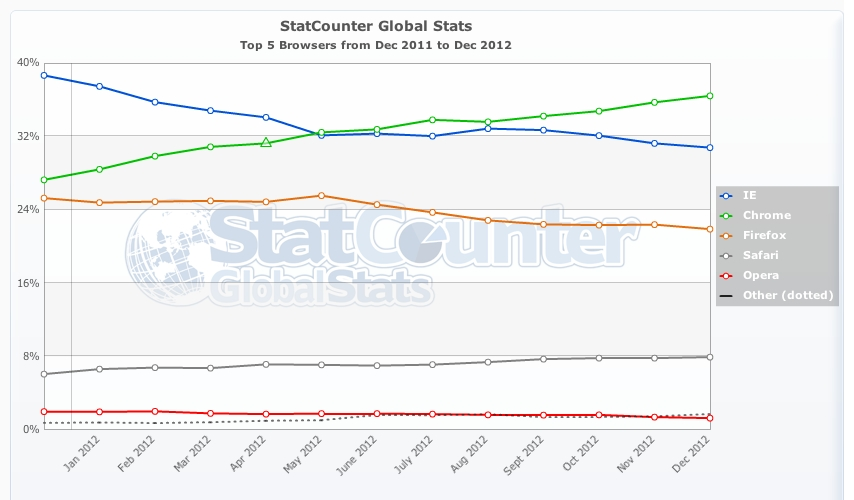
\includegraphics[scale=0.5]{assets/statcounter_browser_2011_dec-2012_dec.jpg}%
		\caption[DUMMY]%
		{Böngészők piaci részesedése 2011. december és 2012. decembere között (\cite{statcounter_browser})}%
		\label{fig:statcounter_browser}
\end{figure}

Azonban más cégek, mint például a github, nem hat hetente ad ki új verziót, hanem a négy hónap alatt huszonöt új verziót tettek elérhetővé (\cite{github_deployment_windows}). Ilyen gyakori kiadási ciklus, csak úgy valósítható meg, ha a legtöbb folyamat automatizálásra kerül (mint ahogy a github automatizálja is), mert ezáltal szinte kizárják az emberi hanyagság okozta hibákat, illetve erőforrást képesek spórolni.


